\newpage
\setcounter{figure}{0}

\section{Rezultati} % (fold)
\label{sec:Rezultati}

U ovom poglavlju su prikazani rezultati izgradnje i ispitana je
funkcionalnost izgradnje 3D modela scena pomoću 3D kamere.  Tijekom
izrade diplomskog rada snimljeno je šest scena RGBDSlam programom i iz
tih snimaka (slika~\ref{fig:01-all.png}) izgrađeni su 3D modeli objekata
i scena upotrebom \texttt{mesh-reconstruction} programa.  Sve snimke i
izrađeni modeli nalaze se na priloženom DVDu.  Za ispitivanje
funkcionalnosti metode odabrane su tri scene:
\texttt{etfos-ured-2013-07-30}, \texttt{etfos-hol-2013-11-20},
\texttt{etfos-hodnik-11-27}. Prije prikaza rezultata potrebno je
istaknuti nekoliko problema odnosno ograničenja ove metode.

Proces snimanja scena RGBDSlam programom odnosno akvizicije oblaka
točaka je obilježen s par problema i ograničenja. Program se nekoliko
puta srušio tijekom snimanja te su snimljeni podaci bili izgubljeni.
Ustanovljeno je da se RBGSlam sruši ako je u ručnom načinu rada te se
pritisne tipka \texttt{Backspace} koja bi trebala obrisati zadnju uzetu
sliku. Također prilikom snimanja pažljivo je odabran "put" snimanja
svake scene kako bi program uspješno mogao spariti značajke s prethodnim
slikama te na kraju zatvoriti petlju i ispraviti akumulirane greške.
Naime, slike moraju biti snimane tako da se scene prikazane na uzastopno
snimljenim slikama djelom preklapaju, kako bi program mogao detektirati
značajke koje su zajedničke tim slikama te na temelju njih odrediti
pomak kamere. Unatoč tome kao što se vidi među rezultatima na nekim
mjestima program nije uspješno spario značajke niti je zatvorio petlju.

Proces izgradnje 3D modela scene \texttt{mesh-reconstruction} programom
obilježen je ograničenjem Poisson algoritma. Algoritam spaja odnosno
popunjava regije/rupe bez točaka u modelu. Isto tako implementacija
algoritma u PCL biblioteci ne uzima u obzir informaciju o boji prilikom
izgradnje modela.

\begin{figure}[h]
\centering
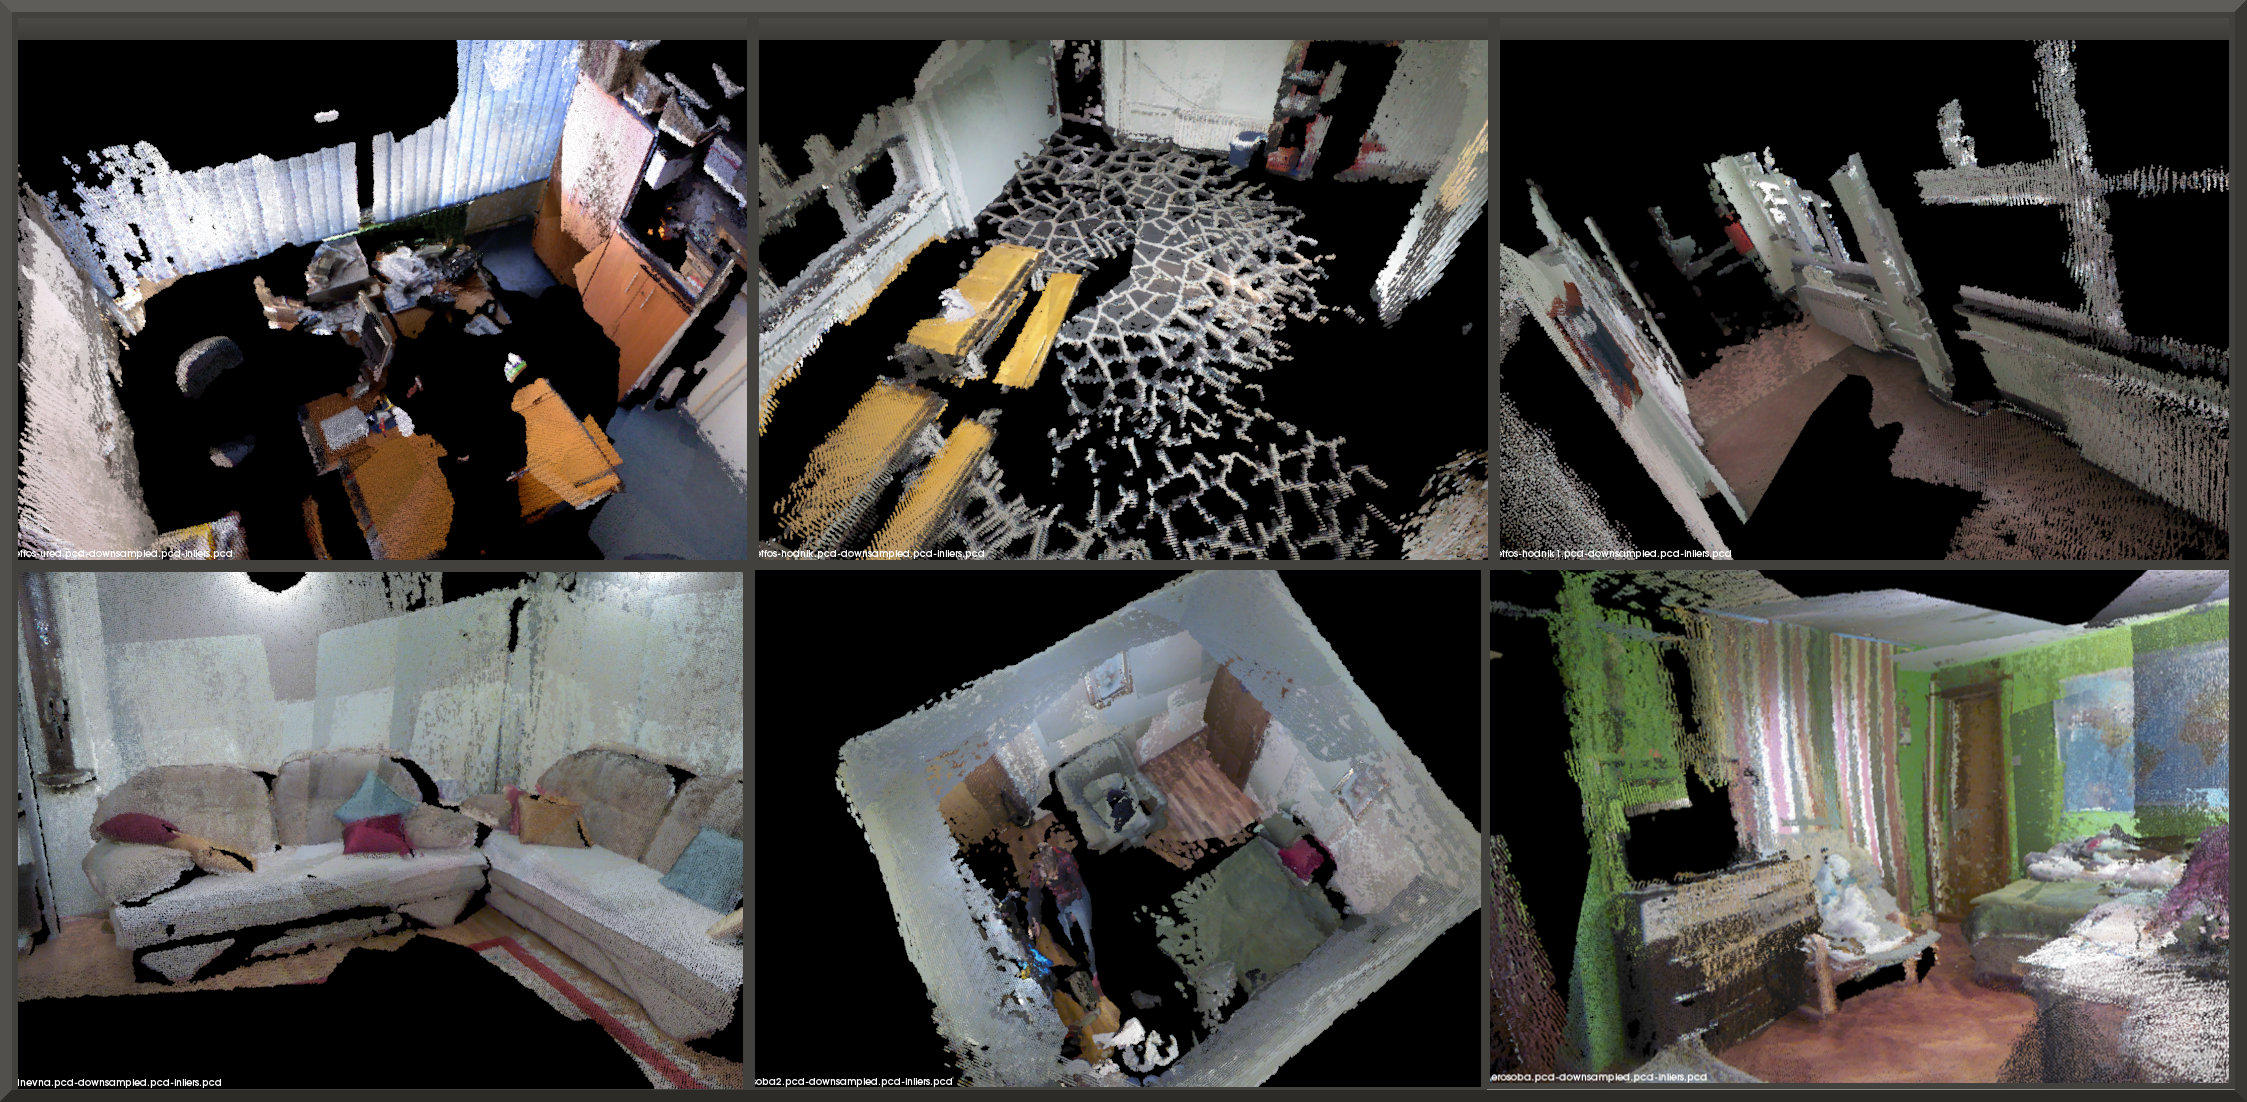
\includegraphics[scale=0.20]{figures/01-all-pcd.png}
\caption{Prikaz svih snimljenih scena}
\label{fig:01-all.png}
\end{figure}

\newpage
\subsection{Prikaz izgrađenih modela scena i objekata} % (fold)
\label{sub:Prikaz izgradenih modela scena i objekata}

Za prikazivanje izrađenih modela scena i oblaka točaka upotrebljen je
komandnolinijski program \texttt{pcl\_viewer} koji ima opciju usporednog
prikazivanja više izgrađenih modela i oblaka točaka iz istog kuta
gledanja. Također program ima mogućnost predočavanja izgrađenih modela
površinom (svi modeli na slici~\ref{fig:etfos-ured}) kao i mrežom
trokuta.

\begin{figure}[h]
\centering
\includegraphics[scale=0.25]{figures/02-etfos-ured-vtk-pcd-all.png}
\caption{Prikaz izrađene mreže trokuta (lijevo) i snimljenog oblaka točaka
(desno) \texttt{etfos-ured-2013-07-30}}
\label{fig:etfos-ured}
\end{figure}

Slika~\ref{fig:etfos-ured} prikazuje izrađenu mrežu trokuta i snimljeni
oblak točaka iz tri različita kuta. Oblak točaka u okolini stola ima
veliku količinu rupa odnosno regija bez točaka. Ta su mjesta u mreži
trokuta popunjena ali zbog nedostatka informacije ne prikazuju stvarno
stanje. Predmeti poput zida, ormara, stola i stolice u prostoriji koji
su adekvatno predočeni u oblaku točaka su isto tako prepoznatljivi i u
izrađenoj mreži trokuta.

\newpage
\begin{figure}[h]
\centering
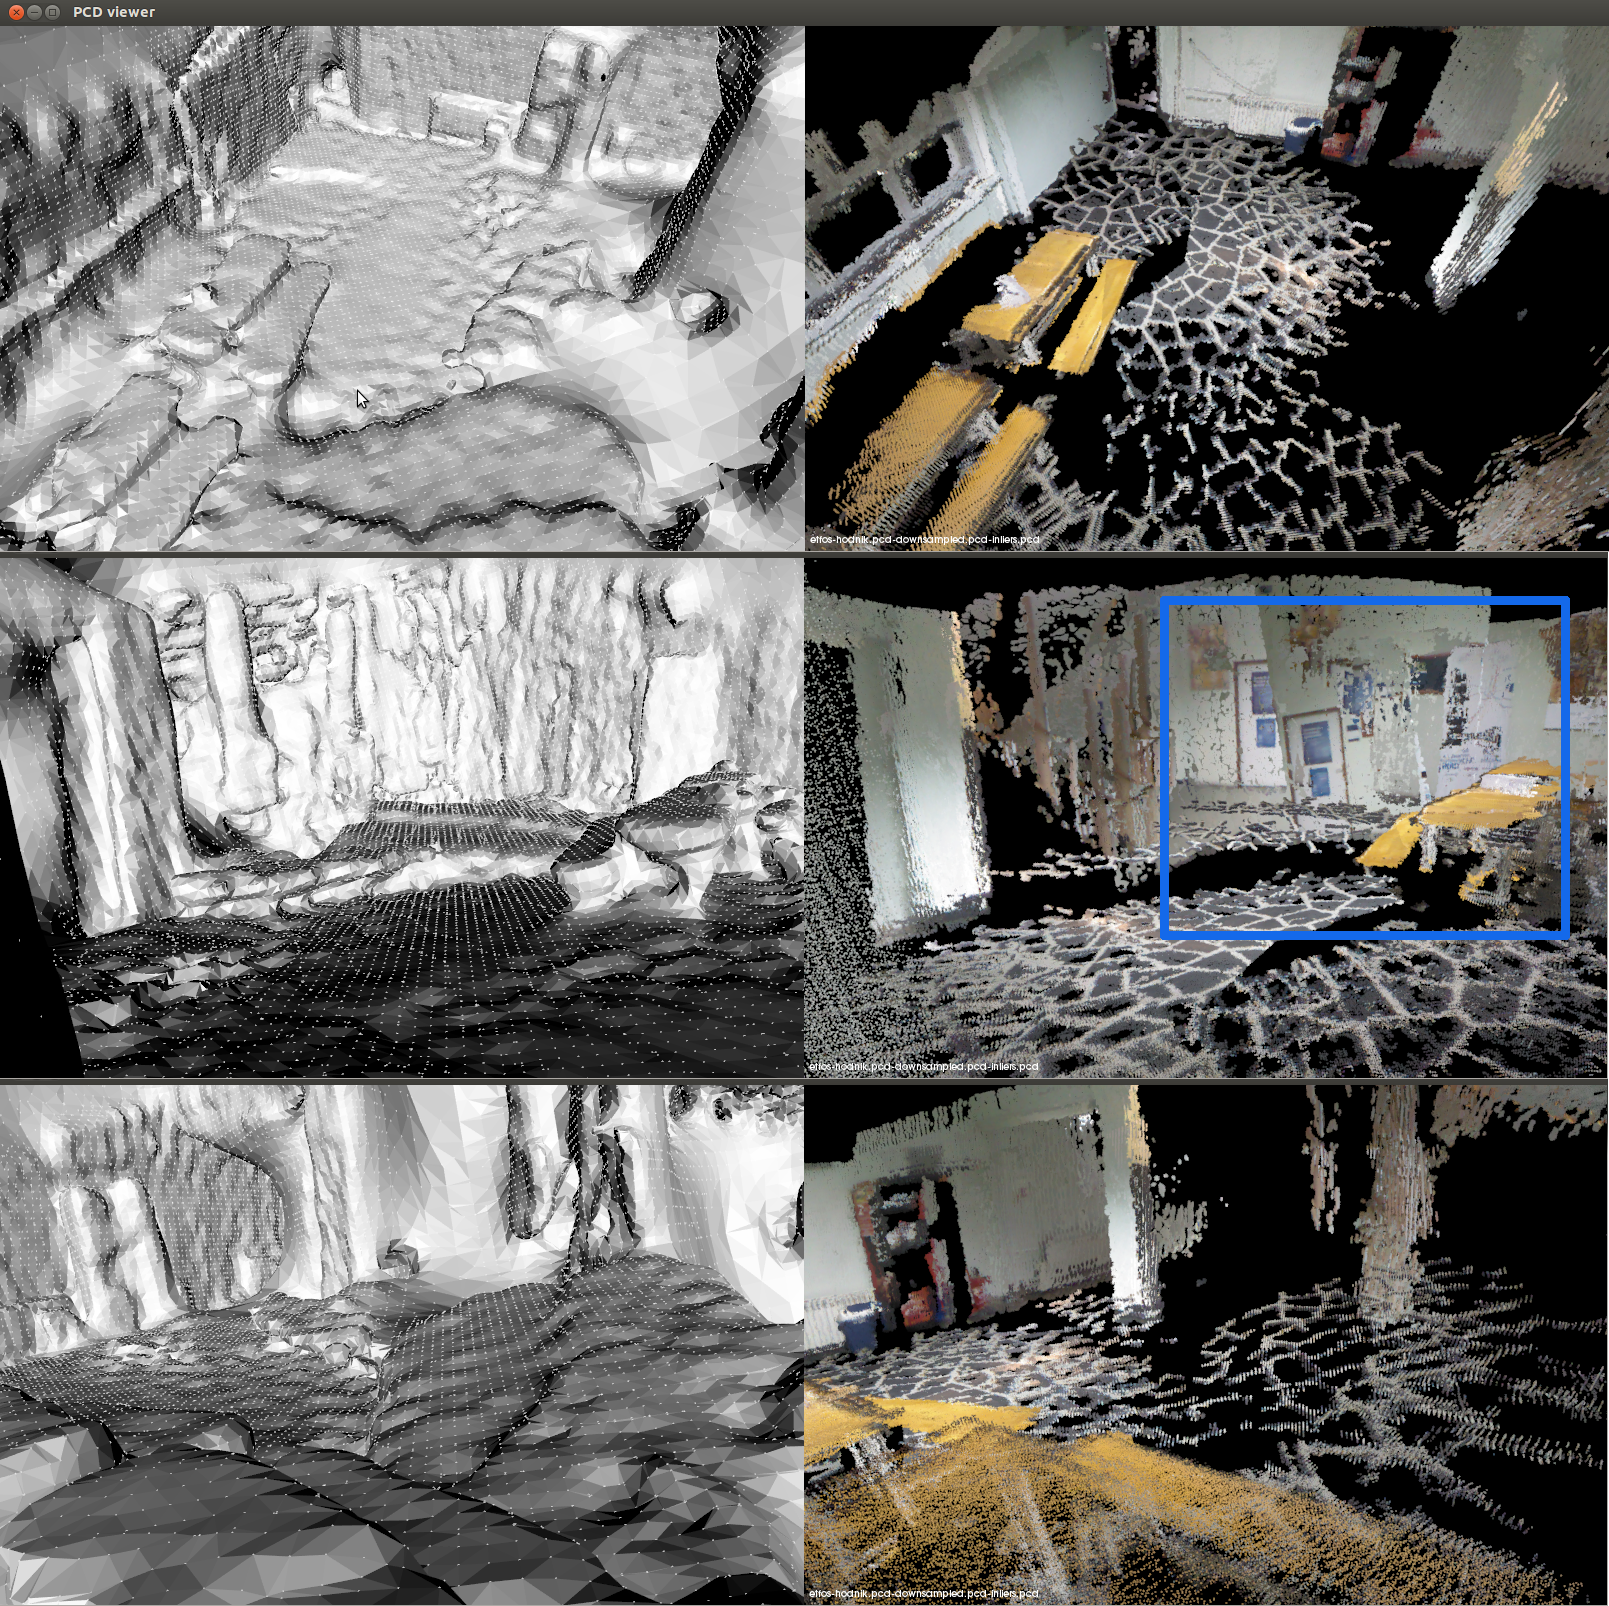
\includegraphics[scale=0.25]{figures/03-etfos-hol-vtk-pcd-all.png}
\caption{Prikaz izrađene mreže trokuta (lijevo) i snimljenog obalka točaka
(desno) \texttt{etfos-hol-2013-11-20}}
\label{fig:etfos-hol}
\end{figure}

Snimanje oblaka točaka na sceni sa slike~\ref{fig:etfos-hol} obilježeno
je neuspješnim zatvaranjem petlje koje je rezultiralo krivim
preklapanjem istih snimki (označeno plavim pravokutnikom). Razlog tome
neuspješno je povezivanje zapaženih orijentira jer je scena "monotona",
s malom količinom detalja, s jednoličnim stepeništem na visinskoj
razlici i fraktalnim uzorkom pločica. Takav oblak točaka iskorišten je
za izgradnju modela što se jasno vidi po odstupanju nivoa poda.
Preostali dio scene uspješno je snimljen i izgrađen.

\newpage
\begin{figure}[h]
\centering
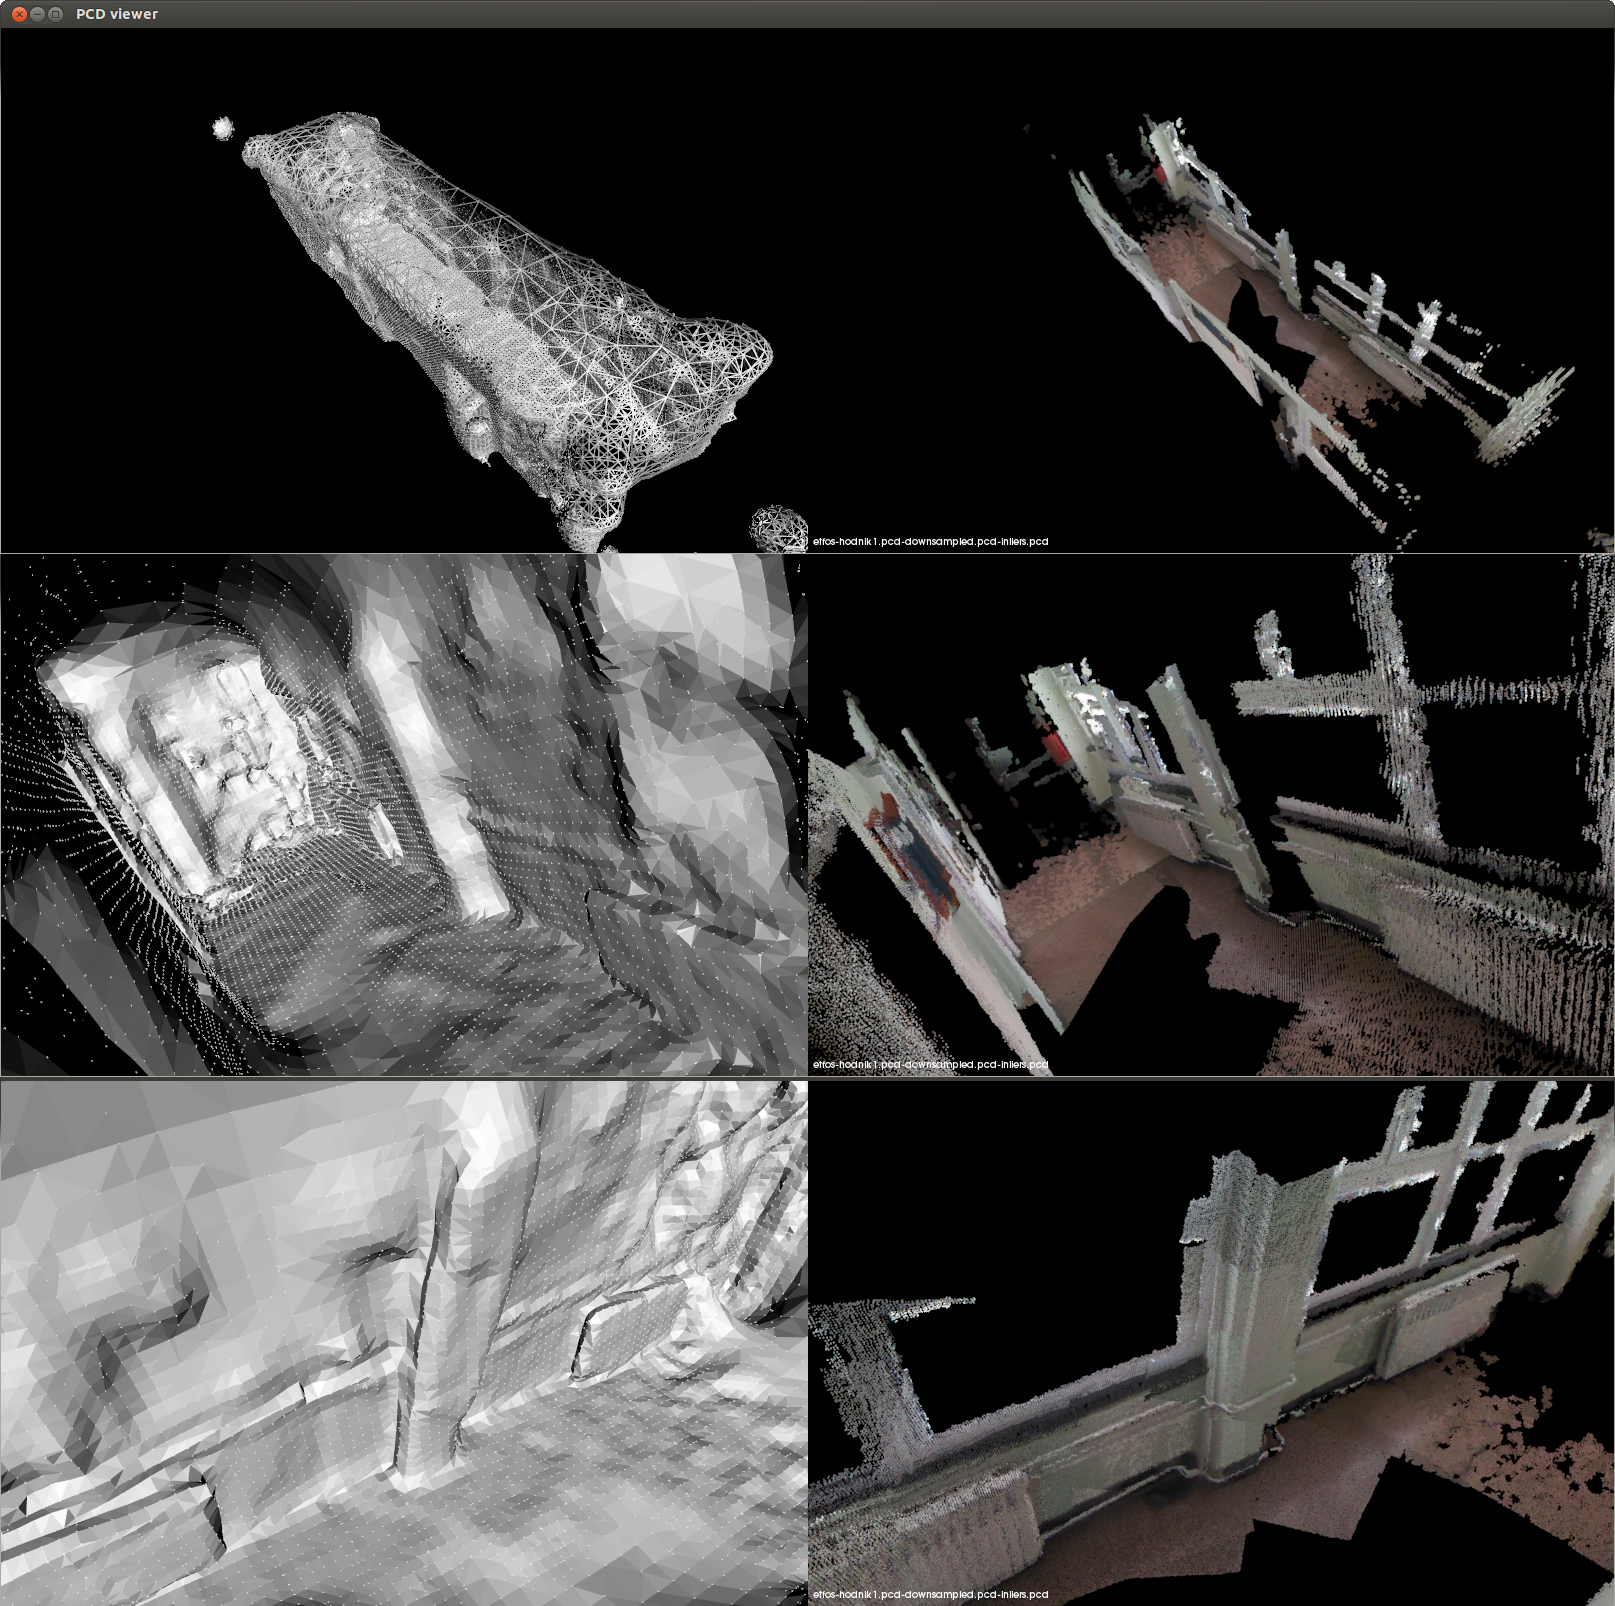
\includegraphics[scale=0.25]{figures/04-etfos-hodnik1-vtk-pcd-all.png}
\caption{Prikaz izrađene mreže trokuta (lijevo) i snimljenog oblaka točaka
(desno) \texttt{etfos-hodnik-2013-11-27}} 
\label{fig:etfos-hodnik}
\end{figure}

Snimanje scene \texttt{etfos-hodnik-2013-11-27} uspješno je izvršeno i
program je izradio oblak točaka. Kao što je i očekivano staklene
površine nisu prikazane jer ne reflektiraju IR zrake. Izrađeni model sa
slike~\ref{fig:etfos-hodnik} dobro prikazuje ograničenje Poisson
algoritma. Primjer ograničenja metode je izrađivanje mreže trokuta po
stropu hodnika. Iako očekivan takav rezultat je nepoželjan. Moguće
poboljšanje algoritma bi bilo da ne izrađuje mrežu troukuta na velikim
rupama. Ovo svojstvo Poisson algoritma, koje u navedenom primjeru daje
neželjeni učinak, u nekim drugim slučajevima daje poželjan rezultat.
Primjer je izrađivanje mreže trokuta po prozorima i drugim manjim rupama
bez točka. Takvo zatvaranje površina je poželjno i na ovoj sceni
uspješno odrađeno.

% subsection Prikaz izgrađenih modela scena i objekata (end)

% section Rezultati (end)

